% Options for packages loaded elsewhere
\PassOptionsToPackage{unicode}{hyperref}
\PassOptionsToPackage{hyphens}{url}
%
\documentclass[
]{article}
\usepackage{lmodern}
\usepackage{amssymb,amsmath}
\usepackage{ifxetex,ifluatex}
\ifnum 0\ifxetex 1\fi\ifluatex 1\fi=0 % if pdftex
  \usepackage[T1]{fontenc}
  \usepackage[utf8]{inputenc}
  \usepackage{textcomp} % provide euro and other symbols
\else % if luatex or xetex
  \usepackage{unicode-math}
  \defaultfontfeatures{Scale=MatchLowercase}
  \defaultfontfeatures[\rmfamily]{Ligatures=TeX,Scale=1}
\fi
% Use upquote if available, for straight quotes in verbatim environments
\IfFileExists{upquote.sty}{\usepackage{upquote}}{}
\IfFileExists{microtype.sty}{% use microtype if available
  \usepackage[]{microtype}
  \UseMicrotypeSet[protrusion]{basicmath} % disable protrusion for tt fonts
}{}
\makeatletter
\@ifundefined{KOMAClassName}{% if non-KOMA class
  \IfFileExists{parskip.sty}{%
    \usepackage{parskip}
  }{% else
    \setlength{\parindent}{0pt}
    \setlength{\parskip}{6pt plus 2pt minus 1pt}}
}{% if KOMA class
  \KOMAoptions{parskip=half}}
\makeatother
\usepackage{xcolor}
\IfFileExists{xurl.sty}{\usepackage{xurl}}{} % add URL line breaks if available
\IfFileExists{bookmark.sty}{\usepackage{bookmark}}{\usepackage{hyperref}}
\hypersetup{
  pdftitle={Assigment3Ver2},
  pdfauthor={Renato Erazo},
  hidelinks,
  pdfcreator={LaTeX via pandoc}}
\urlstyle{same} % disable monospaced font for URLs
\usepackage[margin=1in]{geometry}
\usepackage{color}
\usepackage{fancyvrb}
\newcommand{\VerbBar}{|}
\newcommand{\VERB}{\Verb[commandchars=\\\{\}]}
\DefineVerbatimEnvironment{Highlighting}{Verbatim}{commandchars=\\\{\}}
% Add ',fontsize=\small' for more characters per line
\usepackage{framed}
\definecolor{shadecolor}{RGB}{248,248,248}
\newenvironment{Shaded}{\begin{snugshade}}{\end{snugshade}}
\newcommand{\AlertTok}[1]{\textcolor[rgb]{0.94,0.16,0.16}{#1}}
\newcommand{\AnnotationTok}[1]{\textcolor[rgb]{0.56,0.35,0.01}{\textbf{\textit{#1}}}}
\newcommand{\AttributeTok}[1]{\textcolor[rgb]{0.77,0.63,0.00}{#1}}
\newcommand{\BaseNTok}[1]{\textcolor[rgb]{0.00,0.00,0.81}{#1}}
\newcommand{\BuiltInTok}[1]{#1}
\newcommand{\CharTok}[1]{\textcolor[rgb]{0.31,0.60,0.02}{#1}}
\newcommand{\CommentTok}[1]{\textcolor[rgb]{0.56,0.35,0.01}{\textit{#1}}}
\newcommand{\CommentVarTok}[1]{\textcolor[rgb]{0.56,0.35,0.01}{\textbf{\textit{#1}}}}
\newcommand{\ConstantTok}[1]{\textcolor[rgb]{0.00,0.00,0.00}{#1}}
\newcommand{\ControlFlowTok}[1]{\textcolor[rgb]{0.13,0.29,0.53}{\textbf{#1}}}
\newcommand{\DataTypeTok}[1]{\textcolor[rgb]{0.13,0.29,0.53}{#1}}
\newcommand{\DecValTok}[1]{\textcolor[rgb]{0.00,0.00,0.81}{#1}}
\newcommand{\DocumentationTok}[1]{\textcolor[rgb]{0.56,0.35,0.01}{\textbf{\textit{#1}}}}
\newcommand{\ErrorTok}[1]{\textcolor[rgb]{0.64,0.00,0.00}{\textbf{#1}}}
\newcommand{\ExtensionTok}[1]{#1}
\newcommand{\FloatTok}[1]{\textcolor[rgb]{0.00,0.00,0.81}{#1}}
\newcommand{\FunctionTok}[1]{\textcolor[rgb]{0.00,0.00,0.00}{#1}}
\newcommand{\ImportTok}[1]{#1}
\newcommand{\InformationTok}[1]{\textcolor[rgb]{0.56,0.35,0.01}{\textbf{\textit{#1}}}}
\newcommand{\KeywordTok}[1]{\textcolor[rgb]{0.13,0.29,0.53}{\textbf{#1}}}
\newcommand{\NormalTok}[1]{#1}
\newcommand{\OperatorTok}[1]{\textcolor[rgb]{0.81,0.36,0.00}{\textbf{#1}}}
\newcommand{\OtherTok}[1]{\textcolor[rgb]{0.56,0.35,0.01}{#1}}
\newcommand{\PreprocessorTok}[1]{\textcolor[rgb]{0.56,0.35,0.01}{\textit{#1}}}
\newcommand{\RegionMarkerTok}[1]{#1}
\newcommand{\SpecialCharTok}[1]{\textcolor[rgb]{0.00,0.00,0.00}{#1}}
\newcommand{\SpecialStringTok}[1]{\textcolor[rgb]{0.31,0.60,0.02}{#1}}
\newcommand{\StringTok}[1]{\textcolor[rgb]{0.31,0.60,0.02}{#1}}
\newcommand{\VariableTok}[1]{\textcolor[rgb]{0.00,0.00,0.00}{#1}}
\newcommand{\VerbatimStringTok}[1]{\textcolor[rgb]{0.31,0.60,0.02}{#1}}
\newcommand{\WarningTok}[1]{\textcolor[rgb]{0.56,0.35,0.01}{\textbf{\textit{#1}}}}
\usepackage{graphicx,grffile}
\makeatletter
\def\maxwidth{\ifdim\Gin@nat@width>\linewidth\linewidth\else\Gin@nat@width\fi}
\def\maxheight{\ifdim\Gin@nat@height>\textheight\textheight\else\Gin@nat@height\fi}
\makeatother
% Scale images if necessary, so that they will not overflow the page
% margins by default, and it is still possible to overwrite the defaults
% using explicit options in \includegraphics[width, height, ...]{}
\setkeys{Gin}{width=\maxwidth,height=\maxheight,keepaspectratio}
% Set default figure placement to htbp
\makeatletter
\def\fps@figure{htbp}
\makeatother
\setlength{\emergencystretch}{3em} % prevent overfull lines
\providecommand{\tightlist}{%
  \setlength{\itemsep}{0pt}\setlength{\parskip}{0pt}}
\setcounter{secnumdepth}{-\maxdimen} % remove section numbering

\title{Assigment3Ver2}
\author{Renato Erazo}
\date{1/11/2020}

\begin{document}
\maketitle

\hypertarget{introduction}{%
\subsection{Introduction}\label{introduction}}

Download the le ProgAssignment3-data.zip le containing the data for
Programming Assignment 3 from the Coursera web site. Unzip the le in a
directory that will serve as your working directory. When you start up R
make sure to change your working directory to the directory where you
unzipped the data. The data for this assignment come from the Hospital
Compare web site (\url{http://hospitalcompare.hhs.gov}) run by the U.S.
Department of Health and Human Services. The purpose of the web site is
to provide data and information about the quality of care at over 4,000
Medicare-certied hospitals in the U.S. This dataset es- sentially
covers all major U.S. hospitals. This dataset is used for a variety of
purposes, including determining whether hospitals should be ned for not
providing high quality care to patients (see \url{http://goo.gl/jAXFX}
for some background on this particular topic). The Hospital Compare web
site contains a lot of data and we will only look at a small subset for
this assignment. The zip le for this assignment contains three les •
outcome-of-care-measures.csv: Contains information about 30-day
mortality and readmission rates for heart attacks, heart failure, and
pneumonia for over 4,000 hospitals. • hospital-data.csv: Contains
information about each hospital. • Hospital\_Revised\_Flatfiles.pdf:
Descriptions of the variables in each le (i.e the code book). A
description of the variables in each of the les is in the included PDF
le named Hospital\_Revised\_Flatfiles.pdf. This document contains
information about many other les that are not included with this
programming assignment. You will want to focus on the variables for
Number 19 (\Outcome of Care Measures.csv``) and Number 11
(\Hospital Data.csv''). You may nd it useful to print out this document
(at least the pages for Tables 19 and 11) to have next to you while you
work on this assignment. In particular, the numbers of the variables for
each table indicate column indices in each table (i.e.~\Hospital Name"
is column 2 in the outcome-of-care-measures.csv le).

\hypertarget{read-data}{%
\section{Read data}\label{read-data}}

\hypertarget{read-the-outcome-data-into-r-via-the-read.csv-function-and-look-at-the-frst-few-rows.}{%
\subsubsection{Read the outcome data into R via the read.csv function
and look at the frst few
rows.}\label{read-the-outcome-data-into-r-via-the-read.csv-function-and-look-at-the-frst-few-rows.}}

\begin{Shaded}
\begin{Highlighting}[]
\NormalTok{outcome <-}\StringTok{ }\KeywordTok{read.csv}\NormalTok{(}\StringTok{"outcome-of-care-measures.csv"}\NormalTok{, }\DataTypeTok{colClasses =} \StringTok{"character"}\NormalTok{)}
\KeywordTok{head}\NormalTok{(outcome)}
\end{Highlighting}
\end{Shaded}

\begin{verbatim}
##   Provider.Number                    Hospital.Name                  Address.1
## 1          010001 SOUTHEAST ALABAMA MEDICAL CENTER     1108 ROSS CLARK CIRCLE
## 2          010005    MARSHALL MEDICAL CENTER SOUTH 2505 U S HIGHWAY 431 NORTH
## 3          010006   ELIZA COFFEE MEMORIAL HOSPITAL         205 MARENGO STREET
## 4          010007         MIZELL MEMORIAL HOSPITAL              702 N MAIN ST
## 5          010008      CRENSHAW COMMUNITY HOSPITAL        101 HOSPITAL CIRCLE
## 6          010010    MARSHALL MEDICAL CENTER NORTH    8000 ALABAMA HIGHWAY 69
##   Address.2 Address.3         City State ZIP.Code County.Name Phone.Number
## 1                           DOTHAN    AL    36301     HOUSTON   3347938701
## 2                             BOAZ    AL    35957    MARSHALL   2565938310
## 3                         FLORENCE    AL    35631  LAUDERDALE   2567688400
## 4                              OPP    AL    36467   COVINGTON   3344933541
## 5                          LUVERNE    AL    36049    CRENSHAW   3343353374
## 6                     GUNTERSVILLE    AL    35976    MARSHALL   2565718000
##   Hospital.30.Day.Death..Mortality..Rates.from.Heart.Attack
## 1                                                      14.3
## 2                                                      18.5
## 3                                                      18.1
## 4                                             Not Available
## 5                                             Not Available
## 6                                             Not Available
##   Comparison.to.U.S..Rate...Hospital.30.Day.Death..Mortality..Rates.from.Heart.Attack
## 1                                                No Different than U.S. National Rate
## 2                                                No Different than U.S. National Rate
## 3                                                No Different than U.S. National Rate
## 4                                                           Number of Cases Too Small
## 5                                                           Number of Cases Too Small
## 6                                                           Number of Cases Too Small
##   Lower.Mortality.Estimate...Hospital.30.Day.Death..Mortality..Rates.from.Heart.Attack
## 1                                                                                 12.1
## 2                                                                                 14.7
## 3                                                                                 14.8
## 4                                                                        Not Available
## 5                                                                        Not Available
## 6                                                                        Not Available
##   Upper.Mortality.Estimate...Hospital.30.Day.Death..Mortality..Rates.from.Heart.Attack
## 1                                                                                 17.0
## 2                                                                                 23.0
## 3                                                                                 21.8
## 4                                                                        Not Available
## 5                                                                        Not Available
## 6                                                                        Not Available
##   Number.of.Patients...Hospital.30.Day.Death..Mortality..Rates.from.Heart.Attack
## 1                                                                            666
## 2                                                                             44
## 3                                                                            329
## 4                                                                             14
## 5                                                                              9
## 6                                                                             22
##                                Footnote...Hospital.30.Day.Death..Mortality..Rates.from.Heart.Attack
## 1                                                                                                  
## 2                                                                                                  
## 3                                                                                                  
## 4 number of cases is too small (fewer than 25) to reliably tell how well the hospital is performing
## 5 number of cases is too small (fewer than 25) to reliably tell how well the hospital is performing
## 6 number of cases is too small (fewer than 25) to reliably tell how well the hospital is performing
##   Hospital.30.Day.Death..Mortality..Rates.from.Heart.Failure
## 1                                                       11.4
## 2                                                       15.2
## 3                                                       11.3
## 4                                                       13.6
## 5                                                       13.8
## 6                                                       12.5
##   Comparison.to.U.S..Rate...Hospital.30.Day.Death..Mortality..Rates.from.Heart.Failure
## 1                                                 No Different than U.S. National Rate
## 2                                                        Worse than U.S. National Rate
## 3                                                 No Different than U.S. National Rate
## 4                                                 No Different than U.S. National Rate
## 5                                                 No Different than U.S. National Rate
## 6                                                 No Different than U.S. National Rate
##   Lower.Mortality.Estimate...Hospital.30.Day.Death..Mortality..Rates.from.Heart.Failure
## 1                                                                                   9.5
## 2                                                                                  12.2
## 3                                                                                   9.1
## 4                                                                                  10.0
## 5                                                                                   9.9
## 6                                                                                   9.9
##   Upper.Mortality.Estimate...Hospital.30.Day.Death..Mortality..Rates.from.Heart.Failure
## 1                                                                                  13.7
## 2                                                                                  18.8
## 3                                                                                  13.9
## 4                                                                                  18.2
## 5                                                                                  18.7
## 6                                                                                  15.6
##   Number.of.Patients...Hospital.30.Day.Death..Mortality..Rates.from.Heart.Failure
## 1                                                                             741
## 2                                                                             234
## 3                                                                             523
## 4                                                                             113
## 5                                                                              53
## 6                                                                             163
##   Footnote...Hospital.30.Day.Death..Mortality..Rates.from.Heart.Failure
## 1                                                                      
## 2                                                                      
## 3                                                                      
## 4                                                                      
## 5                                                                      
## 6                                                                      
##   Hospital.30.Day.Death..Mortality..Rates.from.Pneumonia
## 1                                                   10.9
## 2                                                   13.9
## 3                                                   13.4
## 4                                                   14.9
## 5                                                   15.8
## 6                                                    8.7
##   Comparison.to.U.S..Rate...Hospital.30.Day.Death..Mortality..Rates.from.Pneumonia
## 1                                             No Different than U.S. National Rate
## 2                                             No Different than U.S. National Rate
## 3                                             No Different than U.S. National Rate
## 4                                             No Different than U.S. National Rate
## 5                                             No Different than U.S. National Rate
## 6                                                   Better than U.S. National Rate
##   Lower.Mortality.Estimate...Hospital.30.Day.Death..Mortality..Rates.from.Pneumonia
## 1                                                                               8.6
## 2                                                                              11.3
## 3                                                                              11.2
## 4                                                                              11.6
## 5                                                                              11.4
## 6                                                                               6.8
##   Upper.Mortality.Estimate...Hospital.30.Day.Death..Mortality..Rates.from.Pneumonia
## 1                                                                              13.7
## 2                                                                              17.0
## 3                                                                              15.8
## 4                                                                              19.0
## 5                                                                              21.5
## 6                                                                              11.0
##   Number.of.Patients...Hospital.30.Day.Death..Mortality..Rates.from.Pneumonia
## 1                                                                         371
## 2                                                                         372
## 3                                                                         836
## 4                                                                         239
## 5                                                                          61
## 6                                                                         315
##   Footnote...Hospital.30.Day.Death..Mortality..Rates.from.Pneumonia
## 1                                                                  
## 2                                                                  
## 3                                                                  
## 4                                                                  
## 5                                                                  
## 6                                                                  
##   Hospital.30.Day.Readmission.Rates.from.Heart.Attack
## 1                                                19.0
## 2                                       Not Available
## 3                                                17.8
## 4                                       Not Available
## 5                                       Not Available
## 6                                       Not Available
##   Comparison.to.U.S..Rate...Hospital.30.Day.Readmission.Rates.from.Heart.Attack
## 1                                          No Different than U.S. National Rate
## 2                                                     Number of Cases Too Small
## 3                                          No Different than U.S. National Rate
## 4                                                     Number of Cases Too Small
## 5                                                     Number of Cases Too Small
## 6                                                     Number of Cases Too Small
##   Lower.Readmission.Estimate...Hospital.30.Day.Readmission.Rates.from.Heart.Attack
## 1                                                                             16.6
## 2                                                                    Not Available
## 3                                                                             14.9
## 4                                                                    Not Available
## 5                                                                    Not Available
## 6                                                                    Not Available
##   Upper.Readmission.Estimate...Hospital.30.Day.Readmission.Rates.from.Heart.Attack
## 1                                                                             21.7
## 2                                                                    Not Available
## 3                                                                             21.5
## 4                                                                    Not Available
## 5                                                                    Not Available
## 6                                                                    Not Available
##   Number.of.Patients...Hospital.30.Day.Readmission.Rates.from.Heart.Attack
## 1                                                                      728
## 2                                                                       21
## 3                                                                      342
## 4                                                                        1
## 5                                                                        4
## 6                                                                       13
##                                      Footnote...Hospital.30.Day.Readmission.Rates.from.Heart.Attack
## 1                                                                                                  
## 2 number of cases is too small (fewer than 25) to reliably tell how well the hospital is performing
## 3                                                                                                  
## 4 number of cases is too small (fewer than 25) to reliably tell how well the hospital is performing
## 5 number of cases is too small (fewer than 25) to reliably tell how well the hospital is performing
## 6 number of cases is too small (fewer than 25) to reliably tell how well the hospital is performing
##   Hospital.30.Day.Readmission.Rates.from.Heart.Failure
## 1                                                 23.7
## 2                                                 22.5
## 3                                                 19.8
## 4                                                 27.1
## 5                                                 24.7
## 6                                                 23.9
##   Comparison.to.U.S..Rate...Hospital.30.Day.Readmission.Rates.from.Heart.Failure
## 1                                           No Different than U.S. National Rate
## 2                                           No Different than U.S. National Rate
## 3                                                 Better than U.S. National Rate
## 4                                           No Different than U.S. National Rate
## 5                                           No Different than U.S. National Rate
## 6                                           No Different than U.S. National Rate
##   Lower.Readmission.Estimate...Hospital.30.Day.Readmission.Rates.from.Heart.Failure
## 1                                                                              21.3
## 2                                                                              19.2
## 3                                                                              17.2
## 4                                                                              22.4
## 5                                                                              19.9
## 6                                                                              20.1
##   Upper.Readmission.Estimate...Hospital.30.Day.Readmission.Rates.from.Heart.Failure
## 1                                                                              26.5
## 2                                                                              26.1
## 3                                                                              22.9
## 4                                                                              31.9
## 5                                                                              30.2
## 6                                                                              28.2
##   Number.of.Patients...Hospital.30.Day.Readmission.Rates.from.Heart.Failure
## 1                                                                       891
## 2                                                                       264
## 3                                                                       614
## 4                                                                       135
## 5                                                                        59
## 6                                                                       173
##   Footnote...Hospital.30.Day.Readmission.Rates.from.Heart.Failure
## 1                                                                
## 2                                                                
## 3                                                                
## 4                                                                
## 5                                                                
## 6                                                                
##   Hospital.30.Day.Readmission.Rates.from.Pneumonia
## 1                                             17.1
## 2                                             17.6
## 3                                             16.9
## 4                                             19.4
## 5                                             18.0
## 6                                             18.7
##   Comparison.to.U.S..Rate...Hospital.30.Day.Readmission.Rates.from.Pneumonia
## 1                                       No Different than U.S. National Rate
## 2                                       No Different than U.S. National Rate
## 3                                       No Different than U.S. National Rate
## 4                                       No Different than U.S. National Rate
## 5                                       No Different than U.S. National Rate
## 6                                       No Different than U.S. National Rate
##   Lower.Readmission.Estimate...Hospital.30.Day.Readmission.Rates.from.Pneumonia
## 1                                                                          14.4
## 2                                                                          15.0
## 3                                                                          14.7
## 4                                                                          15.9
## 5                                                                          14.0
## 6                                                                          15.7
##   Upper.Readmission.Estimate...Hospital.30.Day.Readmission.Rates.from.Pneumonia
## 1                                                                          20.4
## 2                                                                          20.6
## 3                                                                          19.5
## 4                                                                          23.2
## 5                                                                          22.8
## 6                                                                          22.2
##   Number.of.Patients...Hospital.30.Day.Readmission.Rates.from.Pneumonia
## 1                                                                   400
## 2                                                                   374
## 3                                                                   842
## 4                                                                   254
## 5                                                                    56
## 6                                                                   326
##   Footnote...Hospital.30.Day.Readmission.Rates.from.Pneumonia
## 1                                                            
## 2                                                            
## 3                                                            
## 4                                                            
## 5                                                            
## 6
\end{verbatim}

\begin{Shaded}
\begin{Highlighting}[]
\NormalTok{outcome <-}\StringTok{ }\KeywordTok{read.csv}\NormalTok{(}\StringTok{"outcome-of-care-measures.csv"}\NormalTok{)}
\end{Highlighting}
\end{Shaded}

There are many columns in this dataset. You can see how many by typing
ncol(outcome) (you can see the number of rows with the nrow function).
In addition, you can see the names of each column by typing
names(outcome) (the names are also in the PDF document. To make a simple
histogram of the 30-day death rates from heart attack (column 11 in the
outcome dataset), run.

Because we originally read the data in as character (by specifying
colClasses = ``character'' we need to coerce the column to be numeric.
You may get a warning about NAs being introduced but that is okay.

\begin{Shaded}
\begin{Highlighting}[]
\NormalTok{outcome[,}\DecValTok{11}\NormalTok{] <-}\StringTok{ }\KeywordTok{as.numeric}\NormalTok{(outcome[,}\DecValTok{11}\NormalTok{])}
\end{Highlighting}
\end{Shaded}

\begin{verbatim}
## Warning: NAs introducidos por coerción
\end{verbatim}

\begin{Shaded}
\begin{Highlighting}[]
\KeywordTok{hist}\NormalTok{(outcome[,}\DecValTok{11}\NormalTok{])}
\end{Highlighting}
\end{Shaded}

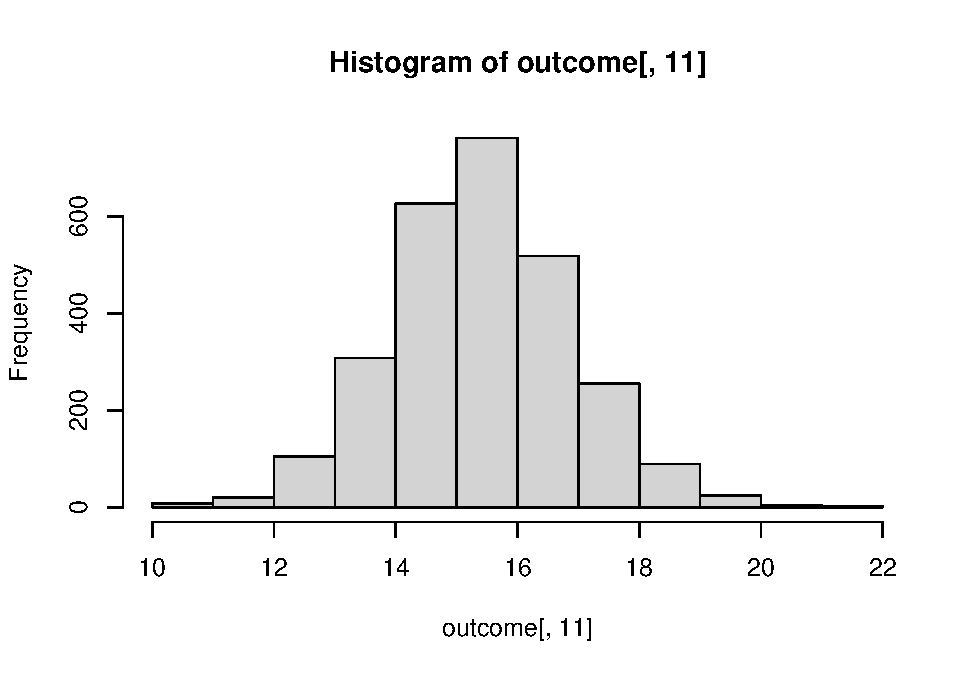
\includegraphics{Assigment3Ver2_files/figure-latex/unnamed-chunk-3-1.pdf}

\hypertarget{finding-the-best-hospital-in-a-state}{%
\subsection{2 Finding the best hospital in a
state}\label{finding-the-best-hospital-in-a-state}}

Write a function called best that take two arguments: the 2-character
abbreviated name of a state and an outcome name. The function reads the
outcome-of-care-measures.csv file and returns a character vector with
the name of the hospital that has the best (i.e.~lowest) 30-day
mortality for the specified outcome in that state. The hospital name is
the name provided in the Hospital.Name variable. The outcomes can be one
of \heart attack``, \heart failure'', or \pneumonia". Hospitals that do
not have data on a particular outcome should be excluded from the set of
hospitals when deciding the rankings.

Handling ties. If there is a tie for the best hospital for a given
outcome, then the hospital names should be sorted in alphabetical order
and the frst hospital in that set should be chosen (i.e.~if hospitals
\b", \c", and \f" are tied for best, then hospital \b" should be
returned).

\#Funcions para validar datos de entrada

\begin{Shaded}
\begin{Highlighting}[]
\KeywordTok{library}\NormalTok{(}\StringTok{"stringi"}\NormalTok{)}
\end{Highlighting}
\end{Shaded}

\begin{verbatim}
## Warning: package 'stringi' was built under R version 4.0.3
\end{verbatim}

\begin{Shaded}
\begin{Highlighting}[]
\NormalTok{validar <-}\ControlFlowTok{function}\NormalTok{(ds,s,r)}
\NormalTok{\{}
  \CommentTok{## To Propercase}
 \CommentTok{# if ("package:stringi" %in% search())}
  \CommentTok{#\{}
   \CommentTok{# install.packages("stringi")}
  \CommentTok{#\}}
  \KeywordTok{require}\NormalTok{(stringi)}
  
\NormalTok{  r <-}\StringTok{ }\KeywordTok{stri_trans_general}\NormalTok{(r, }\DataTypeTok{id =} \StringTok{"Title"}\NormalTok{)}
  
  \KeywordTok{print}\NormalTok{(r)}
  
  
  \CommentTok{## Read outcome data}
\NormalTok{  outcome <-}\StringTok{ }\KeywordTok{read.csv}\NormalTok{(ds, }\DataTypeTok{colClasses =} \StringTok{"character"}\NormalTok{)}
  
  \CommentTok{## Check that state and outcome are valid}
  
\NormalTok{  estadoOk <-}\StringTok{ }\KeywordTok{sum}\NormalTok{(}\KeywordTok{sapply}\NormalTok{(outcome}\OperatorTok{$}\NormalTok{State,}\ControlFlowTok{function}\NormalTok{(x) x }\OperatorTok{==}\StringTok{ }\NormalTok{s)) }\OperatorTok{==}\StringTok{ }\DecValTok{0}
  
  \ControlFlowTok{if}\NormalTok{ (estadoOk) \{}
     
      \KeywordTok{stop}\NormalTok{(}\StringTok{'Invalid state'}\NormalTok{)}
\NormalTok{    \}}
  
  
\NormalTok{  tipoRest <-}\StringTok{ }\KeywordTok{c}\NormalTok{(}\StringTok{"Heart Attack"}\NormalTok{, }\StringTok{"Heart Failure"}\NormalTok{, }\StringTok{"Pneumonia"}\NormalTok{)}
\NormalTok{  siTipo <-}\StringTok{ }\KeywordTok{sum}\NormalTok{(}\KeywordTok{sapply}\NormalTok{(tipoRest,}\ControlFlowTok{function}\NormalTok{(x) x }\OperatorTok{==}\StringTok{ }\NormalTok{r)) }\OperatorTok{==}\StringTok{ }\DecValTok{0}
  
  \ControlFlowTok{if}\NormalTok{(siTipo)\{}
   
        \KeywordTok{stop}\NormalTok{(}\StringTok{'Invalid outcome'}\NormalTok{)}
\NormalTok{  \}}
\NormalTok{  outcome}
\NormalTok{\}}
\end{Highlighting}
\end{Shaded}

The function should use the following template.

\begin{Shaded}
\begin{Highlighting}[]
\NormalTok{best <-}\StringTok{ }\ControlFlowTok{function}\NormalTok{ (state, restriccion)}
\NormalTok{\{}
  
\NormalTok{  restriccion <-}\StringTok{ }\KeywordTok{stri_trans_general}\NormalTok{(restriccion, }\DataTypeTok{id =} \StringTok{"Title"}\NormalTok{)}
\NormalTok{  outcome <-}\StringTok{ }\KeywordTok{validar}\NormalTok{(}\DataTypeTok{ds =} \StringTok{"outcome-of-care-measures.csv"}\NormalTok{,}\DataTypeTok{s =}\NormalTok{ state,}\DataTypeTok{r =}\NormalTok{ restriccion)}
  
  
  
  \CommentTok{## Return hospital name in the sate with lowest 30-day death}
  
  \KeywordTok{library}\NormalTok{(dplyr)}
\NormalTok{  prefijo <-}\StringTok{ "Lower.Mortality.Estimate...Hospital.30.Day.Death..Mortality..Rates.from"}
\NormalTok{  indice <-}\StringTok{ }\KeywordTok{sub}\NormalTok{(}\StringTok{" "}\NormalTok{,}\StringTok{"."}\NormalTok{,restriccion)}
\NormalTok{  completo <-}\StringTok{ }\KeywordTok{paste}\NormalTok{(prefijo,indice,}\DataTypeTok{sep =} \StringTok{"."}\NormalTok{)}
\NormalTok{  subOutcome <-}\StringTok{ }\NormalTok{outcome }\OperatorTok\StringTok{ }\KeywordTok{select}\NormalTok{(State,Hospital.Name,completo)}
  
  \CommentTok{## ---- Cambio los nombre de columnas mas simple}
  
  \KeywordTok{names}\NormalTok{(subOutcome) =}\StringTok{ }\KeywordTok{c}\NormalTok{(}\StringTok{"Estado"}\NormalTok{,}\StringTok{"Hospital"}\NormalTok{,}\StringTok{"Data"}\NormalTok{)}
  
  \CommentTok{## --- Solo recuperar datos del estado/provincia seleccionado}
\NormalTok{  subOutcome <-}\StringTok{ }\KeywordTok{subset}\NormalTok{(subOutcome,Estado }\OperatorTok{==}\StringTok{ }\NormalTok{state)}
  
  
 
  
  \CommentTok{#texto a número}

\NormalTok{  subOutcome}\OperatorTok{$}\NormalTok{Data  <-}\StringTok{ }\KeywordTok{as.numeric}\NormalTok{(subOutcome}\OperatorTok{$}\NormalTok{Data)}
  
   \CommentTok{## --- Eliminar NA}
  
\NormalTok{  subOutcome <-}\StringTok{ }\NormalTok{subOutcome }\OperatorTok\StringTok{ }\KeywordTok{filter}\NormalTok{(}\OperatorTok{!}\KeywordTok{is.na}\NormalTok{(Data))}
  
  
  

  \CommentTok{## rate}
  
  
  
  
  
\NormalTok{  subOutcome <-}\StringTok{ }\NormalTok{subOutcome }\OperatorTok\StringTok{ }\KeywordTok{arrange}\NormalTok{(Data)}
  
  \CommentTok{#---- Iterar entre los valores menores}
  
\NormalTok{  mejor <-}\StringTok{ }\NormalTok{subOutcome[}\DecValTok{1}\NormalTok{,}\DecValTok{3}\NormalTok{]}
  
  \CommentTok{# --- Extraere los mejores}
  
\NormalTok{subOutcome }\OperatorTok\StringTok{ }\KeywordTok{filter}\NormalTok{(Data }\OperatorTok{==}\StringTok{ }\NormalTok{mejor) }\OperatorTok\StringTok{ }\KeywordTok{arrange}\NormalTok{(Data)}
  
  
  
\NormalTok{\}}
\end{Highlighting}
\end{Shaded}

\hypertarget{ejemplos}{%
\subsection{----------------- Ejemplos}\label{ejemplos}}

\begin{Shaded}
\begin{Highlighting}[]
\KeywordTok{best}\NormalTok{(}\StringTok{"LA"}\NormalTok{,}\StringTok{"heart Attack"}\NormalTok{)}
\end{Highlighting}
\end{Shaded}

\begin{verbatim}
## [1] "Heart Attack"
\end{verbatim}

\begin{verbatim}
## 
## Attaching package: 'dplyr'
\end{verbatim}

\begin{verbatim}
## The following objects are masked from 'package:stats':
## 
##     filter, lag
\end{verbatim}

\begin{verbatim}
## The following objects are masked from 'package:base':
## 
##     intersect, setdiff, setequal, union
\end{verbatim}

\begin{verbatim}
## Note: Using an external vector in selections is ambiguous.
## i Use `all_of(completo)` instead of `completo` to silence this message.
## i See <https://tidyselect.r-lib.org/reference/faq-external-vector.html>.
## This message is displayed once per session.
\end{verbatim}

\begin{verbatim}
## Warning in best("LA", "heart Attack"): NAs introducidos por coerción
\end{verbatim}

\begin{verbatim}
##   Estado                             Hospital Data
## 1     LA NATCHITOCHES REGIONAL MEDICAL CENTER 10.6
\end{verbatim}

\hypertarget{ranking-hospitals-by-outcome-in-a-state}{%
\subsection{---- 3Ranking hospitals by outcome in a
state}\label{ranking-hospitals-by-outcome-in-a-state}}

Write a function called rankhospital that takes three arguments: the
2-character abbreviated name of a state (state), an outcome (outcome),
and the ranking of a hospital in that state for that outcome (num). The
function reads the outcome-of-care-measures.csv le and returns a
character vector with the name of the hospital that has the ranking
specied by the num argument. For example, the call rankhospital(``MD'',
``heart failure'', 5) would return a character vector containing the
name of the hospital with the 5th lowest 30-day death rate for heart
failure. The num argument can take values \best``, \worst'', or an
integer indicating the ranking (smaller numbers are better). If the
number given by num is larger than the number of hospitals in that
state, then the function should return NA. Hospitals that do not have
data on a particular outcome should be excluded from the set of
hospitals when deciding the rankings. Handling ties. It may occur that
multiple hospitals have the same 30-day mortality rate for a given cause
of death. In those cases ties should be broken by using the hospital
name. For example, in Texas (\TX"), the hospitals with lowest 30-day
mortality rate for heart failure are shown here.

\begin{Shaded}
\begin{Highlighting}[]
\NormalTok{rankhospital <-}\StringTok{ }\ControlFlowTok{function}\NormalTok{(state, outcome, }\DataTypeTok{num =} \StringTok{"best"}\NormalTok{) \{}
  \CommentTok{## Read outcome data}
  \CommentTok{## Check that state and outcome are valid}
  \CommentTok{## Return hospital name in that state with the given rank}
  \CommentTok{## 30-day death rate}
\NormalTok{\}}
\end{Highlighting}
\end{Shaded}

\end{document}
